\documentclass[tikz,border=6pt]{standalone}
\usepackage{amsmath,amssymb}
\usepackage{tikz}
\usetikzlibrary{arrows.meta,calc}

\begin{document}
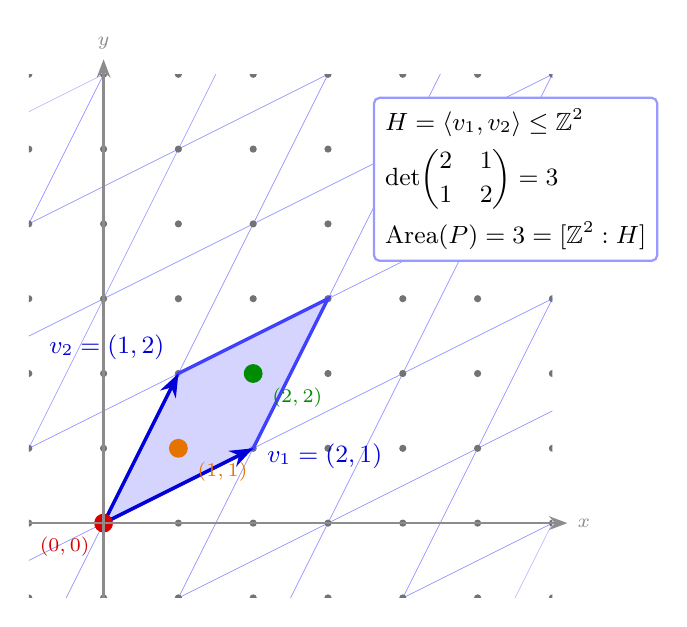
\begin{tikzpicture}[x=0.95cm,y=0.95cm,>=Stealth,thick]

  % Viewport: we will draw a bit beyond and then clip.
  \def\xmin{-1} \def\xmax{6}
  \def\ymin{-1} \def\ymax{6}

  \begin{scope}
    \clip (\xmin,\ymin) rectangle (\xmax,\ymax);

    % --- Tile the plane with translates of the fundamental parallelogram ---
    \def\vax{2} \def\vay{1}
    \def\vbx{1} \def\vby{2}
    \foreach \a in {-3,-2,...,3} {
      \foreach \b in {-3,-2,...,3} {
        \pgfmathsetmacro\ox{\a*\vax + \b*\vbx}
        \pgfmathsetmacro\oy{\a*\vay + \b*\vby}
        \draw[blue!55,very thin,opacity=0.55]
          (\ox,\oy) -- ({\ox+\vax},{\oy+\vay})
          -- ({\ox+\vax+\vbx},{\oy+\vay+\vby})
          -- ({\ox+\vbx},{\oy+\vby}) -- cycle;
      }
    }

    % --- Ambient Z^2 lattice as background dots (on top of tiling) ---
    \foreach \x in {-1,0,...,6} {
      \foreach \y in {-1,0,...,6} {
        \fill[black!55] (\x,\y) circle (1.3pt);
      }
    }

    % --- Highlight the fundamental parallelogram at the origin ---
    \fill[blue!20,opacity=0.85]
      (0,0) -- (\vax,\vay) -- ({\vax+\vbx},{\vay+\vby}) -- (\vbx,\vby) -- cycle;
    \draw[blue!75,very thick]
      (0,0) -- (\vax,\vay) -- ({\vax+\vbx},{\vay+\vby}) -- (\vbx,\vby) -- cycle;

    % --- Basis vectors v1, v2 ---
    \draw[->,blue!85!black,very thick] (0,0) -- (\vax,\vay);
    \draw[->,blue!85!black,very thick] (0,0) -- (\vbx,\vby);

    % --- Coset representatives inside the fundamental parallelogram.
    %     Half-open {αv1+βv2 : α,β ∈ [0,1)} contains exactly (0,0), (1,1), (2,2). ---
    \fill[red!85!black]    (0,0) circle (3.4pt);
    \fill[orange!90!black] (1,1) circle (3.4pt);
    \fill[green!55!black]  (2,2) circle (3.4pt);
  \end{scope}

  % Faint axes (outside the clip so arrowheads stay crisp)
  \draw[->,black!45] (\xmin,0) -- ({\xmax+0.2},0) node[right,font=\scriptsize]{$x$};
  \draw[->,black!45] (0,\ymin) -- (0,{\ymax+0.2}) node[above,font=\scriptsize]{$y$};

  % Vector labels (outside clip so they can overflow slightly if needed)
  \node[blue!85!black,font=\small,anchor=west]       at (2.05,0.90) {$v_1=(2,1)$};
  \node[blue!85!black,font=\small,anchor=south east] at (0.95,2.05) {$v_2=(1,2)$};

  % Coset labels (offset so they don't overlap neighboring lattice dots)
  \node[red!85!black,font=\scriptsize,anchor=north east]    at (-0.05,-0.05) {$(0,0)$};
  \node[orange!90!black,font=\scriptsize,anchor=north west] at ( 1.12, 0.95) {$(1,1)$};
  \node[green!55!black,font=\scriptsize,anchor=north west]  at ( 2.12, 1.95) {$(2,2)$};

  % --- Annotation box ---
  \node[draw=blue!40,fill=white,rounded corners=2pt,inner sep=4pt,
        align=left,anchor=north west,font=\small] at (3.6,5.7) {%
    $H = \langle v_1, v_2\rangle \le \mathbb{Z}^2$\\[3pt]
    $\det\!\begin{pmatrix}2 & 1\\[1pt] 1 & 2\end{pmatrix} = 3$\\[3pt]
    $\mathrm{Area}(P) = 3 = [\mathbb{Z}^2 : H]$};

\end{tikzpicture}
\end{document}
